\chapter{Related Work}
\label{ch:relatedwork}

In this chapter the original work of \citet{chanetal} is presented followed by a simplification of their idea. This simplification serves two purposes: It will be easier to implement which will present a much cleaner code to read and it will be easier to execute since it has much less things to compute and look up. The theory behind a $kD$-tree will also be explained as it is the de facto standard of orthogonal range queries today and will be used to compare the practical results of the simplified model.

\section{kd-trees}

The current standard of range reporting is kd-trees. This technique will be used as a reference point when evaluting the results of the primary work in this thesis. With linear space it is optimal for range reporting on the RAM.

A kd-tree is constructed recursively: Given $n$ points, the median of the points with respect to x are found. All points which has an x-coordinate larger than the median goes to the right child, while points which has an x-coordinate smaller than the median, and the median point, goes to the left child. At the next level the points will be divided in a similar fashion, this time using the y-median and the y-coordinates instead. When dividing $n$ points, the median will be chosen as the $\lceil n/2 \rceil$-th smallest number \cite{compgeo}.
Switching back and forth between focussing on x or y is done at each level of the tree and this will be continued until a binary tree has been constructed with $n$ leaves.

The tree with $n$ points can be represented as flat array with $n$ entries. The $\lceil n/2 \rceil$-th element in the array is the root of the tree.
 With this in mind, the entire tree can represented using a flat array with $n$ elements. 
 \todo{Chapter need work and rework}




\section{Original Range Searching}
\label{sect:original}
Utilizing the \emph{ball-inheritance} concept \citeauthor{chanetal} propose a better solution for ranged search queries. With the same space complexity as the $kD$-tree, but lower query time. Theorem $2.1$ states that \emph{for any $2 \leq B \leq \lg^\epsilon n$, we can can solve $2$-d orthogonal range reporting in rank space with $\mathcal{O}(n \lg_B \lg n)$ space and $(1+k)\mathcal{O}(B \lg \lg n)$ query time.}

First we will look at how ball distributing will work in the ball-inheritance tree and how the ball-inheritance problem can be solved. Then we will show how the ball-inheritance is used in conjunction with other data structures to find the points within a search query $q = [x_1, x_2] \times [y_1, y_2]$.

\subsection{Solving the ball-inheritance problem} 
\label{ssection:solving-ball}

Consider a perfect binary tree with $n$ leaves. At each level a bit vector $A[1..n]$ is used to indicate which of a node's children a ball is inherited by: If $A[i]$ is $0$ means that the ball with identity $i$ in that node was inherited by its left child and $1$ means that it was inherited by its right child. Given a node and an identity of a ball we can know calculate the ball's identity in the node it is inherited by. The node can answer the query $rank(k) = \Sigma_{i \leq k} A[i]$. If a ball is inherited by the right child node its new identity at that node is $rank(i)$ because that is how many $1$'s that preceed it in the current node. If a ball is inherited by the left child node the new identity is then $i-rank(i)$. With this information it is possible to traverse down the tree following a ball from any given node to a leaf. There are $n$ balls per level which is represented by a bit vector of size $n$ bits per level. Even though conceptually this bit vector is divided out amongst the nodes of that level, we can interchangebly think of a bit vector per level or a bit vector per node.\todo{Rephrase and replace} Each level in the tree uses $\mathcal{O}(n)$ bits to store the bit vectors. This adds up to $\mathcal{O}(n \lg n)$ bits, or $\mathcal{O}(n)$ words in all. This trivial solution to the ball-inheritance problem uses $\mathcal{O}(\lg n)$ query time, given that it follows a ball $\mathcal{O}(\lg n)$ steps down to its leaf. The rank function is a constant time query. \\


A bit vector is an array with entries from the alphabet $\Sigma = \{0,1\}$, where each entry is used to indicate whether a left or right child has been chosen to inherit a given ball. By expanding the alphabet we can point to the childrens children, $\Sigma = \{0,1,2,3\}$, the childrens childrens children, $\Sigma = \{0,1,2,3,4,5,6,7\}$, and so forth. Expanding the alphabet will use $\mathcal{O}(n \lg \Sigma)$ bits per level. Storing a pointer from level $i$ to level $i+\Delta$ increases the storage space by $\Delta$ bits per ball, but also enables the ball to be inherited by $2^\Delta$ descendants. By expanding the alphabet the query time can be lowered since it is possible to take bigger steps down the tree. 

Using this concept, we pick $B$ such that $2 \leq B \leq m$. All levels that are a multiple of $B^i$ expand their alphabet such that the balls reach $B^i$ levels down. If a target level does not exist, the ball points to its leaf. We need at most visit $B$ levels that are multiple of $B^i$ before reaching a level that is multiple of $B^{i+1}$, making it possible to jump down the tree with bigger and bigger steps.

Storing the expanded alphabets at each level that is multiple of $B^i$ costs $B^i$ bits per ball. The total cost is then $\Sigma_i \frac{\lg n}{B^i} \cdot \mathcal{O}(B^i) = \mathcal{O}(\lg n \cdot \lg_B \lg n)$ bits per ball (at all levels). With $n$ balls, this is $\mathcal{O}(n \lg_B \lg n)$ words of space with query time of $\mathcal{O}(B \lg_B \lg n)$. \todo{Spørg Kasper med matematikken bag dette - især om ``at all levels'' er rigtig og hvordan $\Sigma$ forvandles til $\lg_B \lg n$}


\subsection{Solving range reporting}
With a solution to the ball-inheritance problem, \citet{chanetal} proposes \textbf{Lemma 2.4} \emph{if the ball inheritance problem can be solved with space $S$ and query time $\tau$, $2$-d range reporting can be solved with space $\mathcal{O}(S+n)$ and query time $\mathcal{O}(\lg \lg n + (1+k) \tau)$.}

Consider a perfect binary tree with $n$ leaves. The root contains $n$ points in $2$-d rank space. These $n$ balls are sorted by their y-rank and will keep this order in all of the nodes in the tree. When distributing the balls for inheritance, a node will give both its children half of its balls: the lower half sorted by the x-rank to its left child and the upper half by x-rank to its right child. The actual coordinates of the balls are only stored at the leaves and we know that x-coordinates of the balls in the leaves are sorted from left to right - smallest to highest. Since the actual coordinate points are only stored once, this data structure uses linear space.

Having distributed the $n$ points from the root to the leaves, additional data structures are required in order to answer the range queries. A succint data structure will be used for the \emph{range minimum query}. Consider an array $A$ with $n$ comparable keys, this data structure allows finding the index of the minimum key in the subarray $A[i,j]$. \todo{Describe either the cartesian tree or reference 29}. For each node in the tree that is a right child a range minimum query structure is added. The indices are the y-rank and the keys are the x-rank that the given node contains. A range maximum query structure is added to the all the nodes which are left children. Each data structure uses $2n + \mathcal{O}(n)$ bits, making it $\mathcal{O}(n)$ bits per level of the tree and $\mathcal{O}(n \lg n)$ bits in all - i.e. $\mathcal{O}(n)$ words of space. This range minimum data structure has a contant query time. \todo{Skal jeg indkludere samme reference som i \citet{chanetal} $[29]$?}\\

There is still the matter of adding predecessor (and successor) search for the y-rank.
For this purpose a succint data structure is added to some levels of the tree. Given a sorted array $A[1..n]$ of $\omega$-bit integers, predecessor search queries in $\mathcal{O}(\lg \omega)$ time is supported using $\mathcal{O}(n \lg \omega)$ space which has oracle access to the entries in the array. \todo{reference}. The points in rank space of $\mathcal{O}(\lg n)$ bits will use $\mathcal{O}(n \lg \lg n)$ bits per level, with $\omega = \lg n$, and $\mathcal{O}(n \lg n \lg \lg n)$ bits in all, which is $\mathcal{O}(n \lg \lg n)$ words. In order to reduce this to linear space we will only place this predecessor search structure at levels which are multiples of $\lg \lg n$. When using the predecessor search from the lowest common ancestor of $x^*_1$ and $x^*_2$, $LCA(x^*_1, x^*_2)$, we go up to the closest ancestor to use its search structure. Searching takes $\mathcal{O}(\lg \lg n)$ time plus $\mathcal{O}(1)$ queries to the ball-inheritance structure: using the ball-inheritance structure we walk at most $\lg \lg n$ steps down while translating the ranks of $y_1$ and $y_2$ to the right and left child of $LCA(x^*_1, x^*_2)$. 

The reason why this structure is necessary for the y-ranks and not the x-ranks, is because of the way the points have been distributed in the ball-inheritance tree: From left to right, the leaves have x-rank $1,2,..n$ so we can easily locate a given range in x-dimension, but in order to keep track of the y-dimensional range we need to follow the balls down the ball-inheritance structure. Adding this structure to each $\lg \lg n$ level saves us from going all the way from the root down to the $LCA$. \todo{rephrase} \\

In order to use this new data structure to report points in the range of $[x_1, x_2] \times [y_1, y_2]$ we follow these steps:
\begin{enumerate}
  \item We find the rank space successor of $x_1$, $x^*_1$, and the rank space predecessor of $x_2$, $x^*_2$. We use these to find the lowest common ancestor of $x^*_1$ and $x^*_2$, $LCA(x^*_1, x^*_2)$. This is the lowest node in the tree containing at least all the points between $x_1$ and $x_2$. By knowing $x^*_1$ and $x^*_2$, finding the lowest common ancestor is a constant time operation. Given that points are in an array, we can use xor as our $LCA$ operation. \todo{rephrase}
  \item As in step $1$ where we found the rank space of the x-coordinates, we find the rank space coordinates of the y-coordinates, $y^*_1$ and $y^*_2$, inside the left and right child of $LCA(x^*_1, x^*_2)$. This step is precisely what the succint data structure mentioned above supports.
  \item We now descend into the right child of $LCA(x^*_1, x^*_2)$ and use the range minimum query structure to the find the index $m$ (the y-rank) of the point with the smallest x-rank in the range $[y^*_1, y^*_2]$. Solving the ball-inheritance problem, we follow the path to the leaf to find the actual x-coordinate of the point. If the x-coordinate is smaller than $x_2$ we return the point as a result and recurse into the ranges of $[y^*_1, m-1]$ and $[m+1, y^*_2]$ in order to find more points. When this is done we apply the same concept to the left child of $LCA(x^*_1, x^*_2)$ using the range maximum query to find points above $x_1$.
\end{enumerate}

\todo{Insert figure to conceptually show we are working our way out from the inside}

The time complexity of step $3$ depends on the use of the ball-inheritance structure. The time to traverse this structure is dependent on the improvements made in \ref{ssection:solving-ball}. An empty range will result in two queries, one query to each child of $LCA(x^*_1, x^*_2)$, otherwise it will not exceed twice the number of nodes beneath $LCA(x^*_1, x^*_2)$. \todo{Why?} Conceptually. $LCA(x^*_1, x^*_2)$ describes a point between $x_1$ and $x_2$. Step $3$ selects points that are in the range of $[y_1, y_2]$ moving outwards from the point of $LCA(x^*_1, x^*_2)$, always picking the point closest to $LCA(x^*_1, x^*_2)$ in its decreasing y-range. \todo{rephrase}

Going back to Lemma $2.4$, we see that the time complexity fits: $\mathcal{O}(\lg \lg n)$ time is used for the predecessor search and $\mathcal{O}((1+k)\tau)$ time is used for walking from the $LCA$ to the leaves solving the ball inheritance problem for the $k$ results.

\section{Simplified Range Searching}

In this section we will describe a simplified model of the one mentioned in section \ref{sect:original}. It mainly uses the ball-inheritance structure. A predecessor search structure will be used a the root of the tree to find the rank space of two points, $(x_1,y_1)$ and $(x_2,y_2)$, delimiting the search range. The algorithm will be described under the assumption that the solution to the ball inheritance problem requires $\mathcal{O}(\lg n)$ query time.
\todo{Nu hvor jeg lige har beskrevet den originale, hvor meget skal jeg så gå i detaljer med hvorfor vi gør tingene? Som f.eks. at have tingene i rank space}

The ball distribution works the same way as it did in the original range searching by \citeauthor{chanetal}: Given a perfect tree with $n$ leaves, the $n$ points are sorted by their y-rank at the root. Distributing its balls, a node will give half of its points to each of its children: the smallest by x-rank to its left child and the highest by x-rank to its right child. The points in the two new lists will retain the same order as the parent. \\

Given a range query $q = [x_1, x_2] \times [y_1, y_2]$ we are going to find the rank successors of $x_1$ and $y_1$ and the rank predecessors of $x_2$ and $y_2$. \todo{Remember to explain why} We call these $x^*_1, y^*_1, x^*_2$ and $y^*_2$. We use $x^*_1$ and $x^*_2$ to find the lowest common ancestor, $LCA(x^*_1, x^*_2)$, containing all the points between $x_1$ and $x_2$. We know the positions of the leaves containing $x^*_1$ and $x^*_2$ so we can traverse from the $LCA$ down to them both. Traversing to $x^*_1$, the first stop is the left child of the $LCA$. From here, each time a node selects its left child as the path to $x^*_1$ we know that the subtree contained in the right child contains points between $x_1$ and $x_2$. Symmetrically, the same applies when going right from the $LCA$: Each time a node selects a right child on the path to $x^*_2$ the subtree contained in the left child contains points between $x_1$ and $x_2$. This concept is seen on figure \ref{fig:LCA}. \\

In the root we mark the position of $y^*_1$ and $y^*_2$ on the bit vector used to indicate which descendant a balls goes to. This range indicates which balls lie within the range of $[y_1, y_2]$. Going forward we will use $i$ and $j$ to indicate this range in the bit vector of any given node. When  a node inherits this range from a parent, the rank function is used to query how many points before $i$ went to this node, and how many points before $j$ went to this node. We refer to section \ref{ssection:solving-ball} on how to update the positions using the rank query. This works because the points in a node are sorted by their y-rank and we keep track of how many points in a given node falls within the range of $[y_1, y_2]$ updating the range of $[i,j]$ everytime a node inherits balls. \\

While keeping the y-rank range updated, we travel from the root to the $LCA$. From here we travel down to all the leafs inside the range of $[x_1, x_2]$ while still updating the y-range. Using the y-range we might be able to decide if we can fully include or fully exclude entire subtrees. We can fully include a subtree if the entire y-rank range of the subtree is within the $[y_1, y_2]$ or fully exclude it if the entire y-range of the subtree falls without $[y_1, y_2]$. Referring to figure \ref{fig:bitvectorsplit} we see how we conceptually update the bit vector and how it would be obvious if the range is either empty or contain the entire subtree. Generalizing this, a leaf can be treated as a subtree: either including or excluding it. \\

\begin{figure}[H]
    \centering
    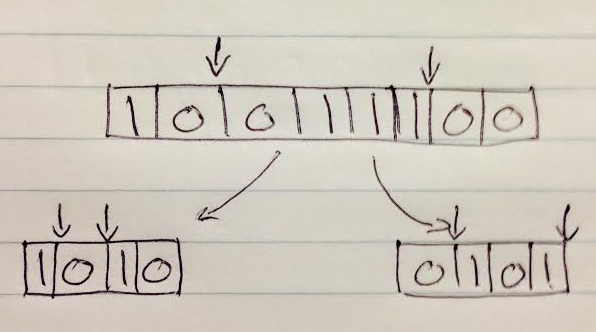
\includegraphics[width=0.6\textwidth]{pictures/bit_vector_split.png}
    \caption{When nodes inherit their bit vector ranges from their parent, it can become obvious if the entire subtree is contained within the range of $[y_1, y_2]$ or falls without the range.}
    \label{fig:bitvectorsplit}
\end{figure}


Summing up, the data structure is utilized as follows:
\begin{enumerate}
    \item Use a binary seach to find the rank space predecessors and successors of $x_1$, $y_1$, $x_2$ and $y_2$. At this point the algorithm will terminate if either rank space range is empty.
    \item From $LCA(x^*_1, x^*_2)$, each leaf between $x^*_1$ and $x^*_2$ will be visited. The range y-rank range found in step $1$ will be updated from the root to this $LCA$ and updated from the $LCA$ to all the leaves visited. When a leaf is visited, its actual coordinates will be reported back as a result.
\end{enumerate}

In order to make the rank query a constant time query, we create a partial rank sum list of the bit vector. Given a bit vector with $n$ bits, the rank at certain intervals is precalculated and stored. Storing the rank at each $32$ bits then enable us to calculate $rank(i)$ by looking up entry $\lfloor \frac{i}{32} \rfloor$ in the partial sum list and summing up $i\% 32$ bits from the bit vector. Calculating the rank thusly takes $\mathcal{O}(1)$ time and requires $\mathcal{O}(n)$ words of space. \todo{Rephrase and maybe move to other chapter} \\

The actual coordinates of the points are only stored at the leaves which then takes up $\mathcal{O}(n)$  words of space. The rest of the tree contains $\lg n$ levels of bit vectors of $n$ bits taking $\mathcal{O}(n \lg n)$ bits, $\mathcal{O}(n)$ words. Looking up the rank-space predecessor and successor of $x_1, x_2, y_1$ and $y_2$ using a simple binary search requires $\mathcal{O}(n)$ space and $\mathcal{O}(\lg n)$ time. Summing it up, the entire data structure uses $\mathcal{O}(n)$ words of space. 

Walking from the root to the $LCA$ requires $\lg n$ steps. Visiting each of the $k$ leaves containing the points which will be reported as a result takes $\mathcal{O}(k \cdot \lg n)$ time.

This adds up to $\mathcal{O}(\lg n + k\cdot\lg n)$ query time to report $k$ points as results. An empty range will be detected by the binary search. If the binary search does not report an empty range, we proceed to use the algorithm, visiting each leaf between $x^*_1$ and $x^*_2$ taking $\mathcal{O}(\lg n)$ time to visit each leaf. \\

\begin{figure}[H]
    \centering
    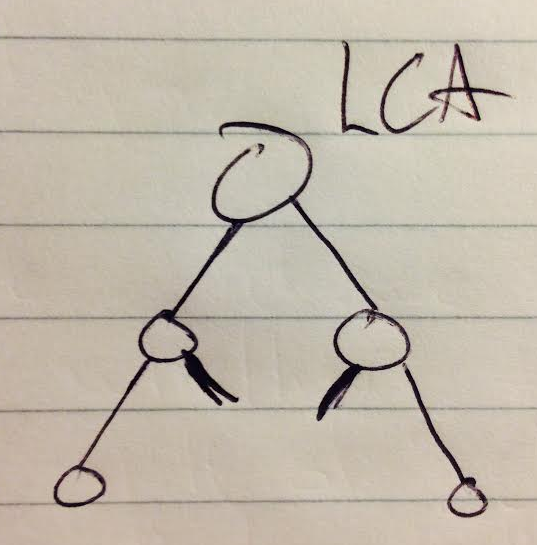
\includegraphics[width=0.6\textwidth]{pictures/LCA.png}
    \caption{Traversing left from the LCA, each right subtree contains x-coordinates between $x_1$ and $x_2$. Traversing right from the LCA the same holds for left subtrees.}
    \label{fig:LCA}
\end{figure}

The three approaches described above all use a number of bits linear to the amount of points. The original search structure by \citet{chanetal} is the fastest with its $(1+k)\mathcal{O}(B\lg \lg n)$ query while kd-trees are the slowest with $\mathcal{O}(\sqrt{n} + k)$ query time.

